\chapter{Lois invariantes, quadrivecteurs et tenseur de champ}

Nous commencerons par une loi que la nature aurait pu respecter, mais qu’elle ne respecte pas. Son échec nous indiquera comment une loi physique doit être écrite. Le même critère conduit d’abord des composantes de coordonnées aux vecteurs ordinaires, puis des vecteurs ordinaires aux quadrivecteurs, et enfin des quadrivecteurs aux tenseurs. À la fin, les champs électrique et magnétique ne seront plus des objets séparés : ensemble, ils occuperont les six composantes indépendantes d’un même tenseur antisymétrique.

Sauf indication contraire, nous utilisons des unités telles que \(c=1\), ordonnons les composantes de l’espace-temps selon \((1,2,3,0)=(x,y,z,t)\) et adoptons la signature métrique \((-,-,-,+)\).

\section{Une loi possible, mais dotée d’une mauvaise symétrie}

Fixons définitivement dans l’espace un axe \(x\) et un axe \(y\). Décidons maintenant que deux particules interagissent dès que leurs coordonnées \(x\) coïncident. L’interaction pourrait inverser leur mouvement ou les envoyer dans de nouvelles directions ; sa dynamique détaillée importe peu. Le déclencheur proposé est simplement \begin{equation}
  x_1-x_2=0,
\end{equation} où les indices désignent les particules, et non les composantes de coordonnées. Cette règle ne présente aucune contradiction mathématique. La question est de savoir ce qui la rend physiquement peu plausible.

\begin{classroomqa}\audiencequestion{La règle viole-t-elle l’homogénéité de l’espace ?}\lecturerresponse{Non. Une translation de l’origine modifie les deux coordonnées de la même quantité et laisse \(x_1-x_2\) inchangé. La règle ne désigne aucun lieu privilégié. Son défaut tient à l’isotropie : elle privilégie une direction.}\end{classroomqa}

Faisons tourner les axes de \(90^\circ\). L’ancienne direction \(x\) s’appelle désormais \(y\) ; les mêmes événements physiques seraient donc décrits par l’égalité des coordonnées \(y\). Pour un angle quelconque, la condition ferait intervenir une combinaison linéaire de \(x\) et de \(y\). La forme de la loi dépend donc de l’orientation du tableau. Elle est invariante par translation, mais pas par rotation.

Nous donnons généralement aux lois physiques leur forme la plus simple dans des coordonnées orthogonales. On peut utiliser des coordonnées plus générales, mais la métrique et les formules deviennent alors moins simples. Au sein de la classe des repères cartésiens orthogonaux, aucune orientation ne doit être privilégiée.

La correction est immédiate. En deux dimensions, exigeons que les deux coordonnées coïncident ; en trois dimensions, exigeons que les trois coïncident : \begin{equation}
  x_1=x_2,
  \qquad y_1=y_2,
  \qquad z_1=z_2.
\end{equation} Les particules ne peuvent alors interagir que lorsqu’elles atteignent le même point, même si elles s’en approchent selon des lignes différentes.

\begin{classroomqa}\audiencequestion{Les coordonnées \(z\) et les temps doivent-ils aussi coïncider ?}\lecturerresponse{Dans l’espace à trois dimensions, les coordonnées \(z\) doivent également coïncider. Pour le moment, nous laissons le temps de côté ; nous le réintroduirons dès que l’argument spatial sera terminé.}\end{classroomqa}

Soit \(\boldsymbol r_a\) la position de la particule \(a\). Les trois conditions sur les composantes se ramènent à une équation vectorielle : \begin{equation}
  \boldsymbol r_1-\boldsymbol r_2=\boldsymbol 0.
\end{equation} Une composante peut s’annuler dans un repère tourné et ne pas s’annuler dans un autre. Le vecteur entier est différent : si toutes ses composantes sont nulles dans un repère, elles le sont dans tous les repères obtenus par rotation. De même, si deux vecteurs sont égaux dans un repère, ils le restent après transformation des deux vecteurs.

\begin{figure}[H]\centering
\includegraphics[width=0.78\textwidth]{lecture_06_figure_01.png}\caption{Les trois égalités de coordonnées qui font de la collision une coïncidence spatiale plutôt qu’une coïncidence le long d’un axe privilégié.}\lectureframe{00:09:00}\end{figure}

Voilà pourquoi les équations vectorielles sont utiles. Leurs composantes changent, mais l’objet se transforme de façon cohérente. Une loi écrite pour l’objet entier peut conserver sa forme lorsque les coordonnées subissent une rotation.

\section{Coïncidence dans l’espace-temps}

Remplaçons maintenant l’axe spatial vertical par le temps. Une règle newtonienne pourrait stipuler que deux changements de mouvement ne se produisent qu’à des instants égaux. En mécanique newtonienne, la simultanéité est la même pour tous les observateurs inertiels ; une telle règle est donc possible. En relativité restreinte, elle sélectionne un référentiel privilégié. Des événements simultanés dans un référentiel ne le sont pas nécessairement dans un autre.

Exiger seulement l’égalité des coordonnées spatiales ne convient pas davantage. Un déplacement dans l’espace-temps peut avoir des composantes spatiales nulles et une composante temporelle non nulle : \begin{equation}
  \Delta X^\mu=(0,0,0,\Delta t),
\end{equation} et un boost mélange \(\Delta t\) avec une composante spatiale. L’énoncé local invariant est que les deux changements de mouvement se produisent au même événement. Ainsi, une collision simple exige \begin{equation}
  X_1^\mu=X_2^\mu,
  \qquad\text{or}\qquad
  X_1^\mu-X_2^\mu=0.
\end{equation} Les quatre coordonnées coïncident : les particules occupent le même lieu au même instant.

L’exemple de la collision fournit une règle générale pour écrire la physique. Nous pouvons tout placer d’un côté et égaler un quadrivecteur complet à zéro, ou égaler un quadrivecteur complet à un autre. Égaler des composantes isolées d’un quadrivecteur ne donne pas, à lui seul, un énoncé invariant de Lorentz.

\section{Boosts, rotations et notation matricielle}

Un quadrivecteur est un objet qui se transforme comme un déplacement dans l’espace-temps. Pour rendre cette définition utile, rappelons d’abord les transformations des coordonnées elles-mêmes. Pour un boost de vitesse \(v\) dans la direction \(x\), \begin{align}
  x'&=\gamma(x-vt), & y'&=y, & z'&=z,
  & t'&=\gamma(t-vx),                                      \label{eq:l6-boost}
\end{align} où \begin{equation}
  \gamma(v)=\frac{1}{\sqrt{1-v^2}}.
\end{equation}

\begin{classroomqa}\audiencequestion{La vitesse de la lumière a-t-elle été posée égale à un dans ces formules ?}\lecturerresponse{Oui. Pour rétablir les unités, prenons \(X^0=ct\), remplaçons \(1-v^2\) par \(1-v^2/c^2\) et réintroduisons les facteurs correspondants de \(c\) dans les termes mêlant espace--temps.}\end{classroomqa}

Une rotation autour de l’axe \(z\) mélange \(x\) et \(y\), tout en laissant \(z\) et \(t\) inchangés : \begin{equation}
\begin{pmatrix}
  x'\\ y'\\ z'\\ t'
\end{pmatrix}
=
\begin{pmatrix}
  \cos\theta & \sin\theta & 0 & 0\\
  -\sin\theta & \cos\theta & 0 & 0\\
  0 & 0 & 1 & 0\\
  0 & 0 & 0 & 1
\end{pmatrix}
\begin{pmatrix}
  x\\ y\\ z\\ t
\end{pmatrix}.
\end{equation} Il vaut la peine d’afficher les zéros : ils indiquent explicitement quelles composantes n’interviennent pas dans la coordonnée transformée considérée. Dans le même ordre, le boost de l’équation~\eqref{eq:l6-boost} s’écrit \begin{equation}
\begin{pmatrix}
  x'\\ y'\\ z'\\ t'
\end{pmatrix}
=
\begin{pmatrix}
  \gamma & 0 & 0 & -\gamma v\\
  0 & 1 & 0 & 0\\
  0 & 0 & 1 & 0\\
  -\gamma v & 0 & 0 & \gamma
\end{pmatrix}
\begin{pmatrix}
  x\\ y\\ z\\ t
\end{pmatrix}.
\end{equation}

On peut composer rotations et boosts par multiplication matricielle. Pour effectuer un boost dans une direction qui n’est pas alignée sur l’axe \(x\) initial, on peut d’abord faire tourner cette direction jusqu’à l’axe \(x\), appliquer le boost, puis effectuer les rotations nécessaires. Les produits de ces matrices élémentaires engendrent des transformations de Lorentz plus générales.

\begin{classroomqa}\audiencequestion{L’ordre importe-t-il : faut-il d’abord faire une rotation puis un boost, ou d’abord un boost puis une rotation ?}\lecturerresponse{Oui. Après la première opération, les axes sur lesquels agit la seconde ont changé. Les deux produits matriciels ne sont pas nécessairement égaux ; l’ordre des opérations importe donc.}\end{classroomqa}

On peut écrire toutes ces transformations linéaires en une seule fois : \begin{equation}
  X'^{\mu}=\Lambda^{\mu}{}_{\nu}X^{\nu}.                  \label{eq:l6-vector-transform}
\end{equation} L’indice répété \(\nu\) est sommé sur \(1,2,3,0\). Il s’agit simplement de la somme habituelle, ligne par colonne, de la multiplication matricielle, exprimée en notation indicielle.

\begin{figure}[H]\centering
\includegraphics[width=0.78\textwidth]{lecture_06_figure_02.png}\caption{La transformation de Lorentz indicielle, au-dessus de son expression sous forme de vecteurs colonnes.}\lectureframe{00:31:55}\end{figure}

L’équation~\eqref{eq:l6-vector-transform} est aussi la définition d’un quadrivecteur contravariant général. Si \(A^\mu\) est un tel vecteur, alors \begin{equation}
  A'^{\mu}=\Lambda^{\mu}{}_{\nu}A^{\nu}.
\end{equation} Ses quatre composantes ne représentent pas nécessairement une position. C’est sa loi de transformation qui fait de cet objet un quadrivecteur.

\section{Scalaires, métrique et produits invariants}

Avant d’utiliser d’autres quadrivecteurs, il est utile de revenir à la notion plus simple de scalaire. Sous les rotations spatiales, la température en un point donné est un scalaire, tout comme la distance entre deux points donnés. Chacun est un nombre unique, indépendant de l’orientation des axes. On pourrait même avancer l’affirmation numérique volontairement absurde qu’une distance mesurée en centimètres est égale à la température ambiante mesurée en degrés Fahrenheit. Cette affirmation n’a aucune portée physique profonde, mais puisque ses deux membres sont des scalaires sous les rotations, sa vérité ou sa fausseté ne dépend pas de la rotation des axes.

Les composantes d’un vecteur ne sont pas des scalaires. Il nous faut donc une méthode systématique pour les combiner en scalaires. Écrivons un quadrivecteur contravariant général sous la forme \begin{equation}
  A^\mu=(A^1,A^2,A^3,A^0).
\end{equation} Les composantes covariantes décrivent le même objet géométrique avec un indice inférieur. Avec notre signature, on les obtient au moyen de la métrique de Minkowski : \begin{equation}
  A_\mu=\eta_{\mu\nu}A^\nu,
  \qquad
  \eta_{\mu\nu}=
  \begin{pmatrix}
    -1&0&0&0\\
    0&-1&0&0\\
    0&0&-1&0\\
    0&0&0&1
  \end{pmatrix},                                          \label{eq:l6-metric}
\end{equation} de sorte que \begin{equation}
  A_\mu=(-A^1,-A^2,-A^3,A^0).
\end{equation}

\begin{classroomqa}\audiencequestion{Y a-t-il deux indices et des signes incohérents au tableau ?}\lecturerresponse{Oui. Il faut ajouter le signe moins correspondant à la composante spatiale de la colonne affichée, et les composantes à droite de l’équation d’abaissement d’indice portent des indices supérieurs avant la multiplication par \(\eta_{\mu\nu}\). L’indice temporel est \(0\), et non \(4\).}\end{classroomqa}

\begin{figure}[H]\centering
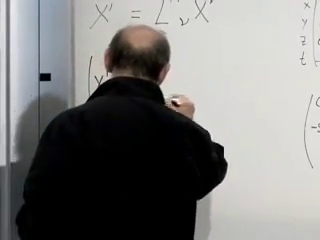
\includegraphics[width=0.8\textwidth]{lecture_06_figure_03.png}\caption{Composantes contravariantes et covariantes, matrice métrique et début de la contraction invariante.}\lectureframe{00:45:00}\end{figure}

L’abaissement d’indice n’est pas une simple convention décorative. Il incorpore les signes nécessaires à la norme invariante de Lorentz : \begin{align}
  A_\mu A^\mu
  &=-(A^1)^2-(A^2)^2-(A^3)^2+(A^0)^2,                    \label{eq:l6-norm}\\
  X_\mu X^\mu
  &=t^2-x^2-y^2-z^2.
\end{align} La seconde expression est l’intervalle d’espace-temps invariant mesuré depuis l’origine. Comme \(A^\mu\) se transforme de la même façon que \(X^\mu\), leur contraction conserve elle aussi son invariance.

La notation nous enseigne également une règle pratique de calcul. Un indice de sommation répété apparaît une fois en position supérieure et une fois en position inférieure. Par exemple, \begin{equation}
  A_\mu A^\mu
  =\eta_{\mu\nu}A^\mu A^\nu.
\end{equation} On peut changer le nom des indices sommés, ou indices muets, sans modifier la quantité.

\begin{classroomqa}\audiencequestion{Faut-il considérer l’un de ces vecteurs comme une ligne et l’autre comme une colonne, et leur ordre importe-t-il ?}\lecturerresponse{Pour le calcul présent, considérons les quantités indicées comme des composantes et laissons la métrique effectuer la contraction ; inutile de ramener la discussion à l’algèbre des opérateurs en lignes et en colonnes. Ce sont des nombres ordinaires, donc leur ordre importe peu. Les opérateurs qui ne commutent pas exigeraient davantage de précautions, mais ce n’est pas le sujet ici.}\end{classroomqa}

La même construction définit un produit scalaire entre deux quadrivecteurs distincts : \begin{equation}
  A\mathbin{\cdot}B=A_\mu B^\mu=A^\mu B_\mu.
\end{equation} Son invariance se démontre sans écrire explicitement une matrice de Lorentz. Puisque \(A+B\) et \(A-B\) sont des quadrivecteurs, leurs normes au carré sont invariantes : \begin{align}
  (A+B)^2&=A^2+B^2+2A\mathbin{\cdot}B,\\
  (A-B)^2&=A^2+B^2-2A\mathbin{\cdot}B.
\end{align} En faisant la différence, on obtient \begin{equation}
  (A+B)^2-(A-B)^2=4A\mathbin{\cdot}B,                    \label{eq:l6-polarization}
\end{equation} ; ainsi \(A\mathbin{\cdot}B\) est également invariant. Le facteur quatre découle directement du développement.\editorialnote{L’argument au tableau donne cette identité de polarisation ; écrire explicitement le facteur lève toute ambiguïté sur la simplification évoquée à l’oral.}

\begin{figure}[H]\centering
\includegraphics[width=0.8\textwidth]{lecture_06_figure_04.png}\caption{Les deux carrés invariants utilisés pour isoler le produit scalaire de quadrivecteurs distincts.}\lectureframe{00:52:20}\end{figure}

Les quantités invariantes sont des ingrédients naturels des lois physiques : contrairement à une composante isolée, elles conservent la même valeur d’un référentiel à l’autre.

\section{Vitesse propre et quadrivecteur énergie-impulsion}

Considérons deux événements voisins sur la ligne d’univers d’une particule. Leur séparation est le quadrivecteur infinitésimal \begin{equation}
  dX^\mu=(dx,dy,dz,dt).
\end{equation} Pour une ligne d’univers de genre temps, le temps propre est défini par \begin{equation}
  d\tau^2=dX_\mu dX^\mu
  =dt^2-dx^2-dy^2-dz^2.                                  \label{eq:l6-proper-time}
\end{equation} Le quadrivecteur vitesse propre est \begin{equation}
  U^\mu=\frac{dX^\mu}{d\tau}.                            \label{eq:l6-four-velocity}
\end{equation} Il mesure le taux de variation de la position dans l’espace-temps par rapport au temps propre de la particule, et non par rapport au temps coordonné d’un référentiel choisi.

Bien que \(U^\mu\) ait quatre composantes, seules trois sont indépendantes. En divisant l’équation~\eqref{eq:l6-proper-time} par \(d\tau^2\), on obtient \begin{equation}
  U_\mu U^\mu=1.
\end{equation} Le quadrivecteur vitesse propre est donc un vecteur unitaire de genre temps. Le choix orienté vers le futur fixe le signe de sa composante temporelle.

\begin{classroomqa}
\audiencequestion{À des vitesses très inférieures à \(c\), la quadrivitesse se réduit-elle à la vitesse ordinaire ?}
\lecturerresponse{Ses trois composantes spatiales tendent vers la vitesse ordinaire, tandis que sa composante temporelle tend vers l’unité dans les unités \(c=1\). Cette relation découle de l’application de la règle de la chaîne et du calcul de \(dt/d\tau\).}
\end{classroomqa}

Pour chaque composante spatiale, \begin{equation}
  U^i=\frac{dx^i}{d\tau}
     =\frac{dx^i}{dt}\frac{dt}{d\tau}
     =v^i\frac{dt}{d\tau}.
\end{equation} Divisons l’équation~\eqref{eq:l6-proper-time} par \(dt^2\) : \begin{equation}
  \left(\frac{d\tau}{dt}\right)^2
  =1-v_x^2-v_y^2-v_z^2
  =1-\boldsymbol v^2.
\end{equation} On en déduit \begin{equation}
  \frac{dt}{d\tau}=\frac{1}{\sqrt{1-\boldsymbol v^2}}
  =\gamma(\lvert\boldsymbol v\rvert),
\end{equation} et \begin{equation}
  U^\mu=(\gamma v_x,\gamma v_y,\gamma v_z,\gamma).
                                                                  \label{eq:l6-u-components}
\end{equation}

\begin{figure}[H]\centering
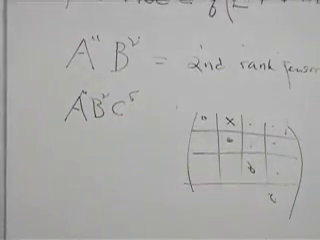
\includegraphics[width=0.8\textwidth]{lecture_06_figure_05.png}\caption{Le calcul du temps propre qui donne \(dt/d\tau=\gamma\) et relie la vitesse propre à la vitesse ordinaire.}\lectureframe{01:02:00}\end{figure}

\begin{classroomqa}\audiencequestion{\(dx^2/dt^2\) désigne-t-il une dérivée seconde, et le carré d’un vecteur doit-il produire des termes croisés ?}\lecturerresponse{Ici, il désigne \((dx/dt)^2\), le carré d’une dérivée première. De plus, \(\boldsymbol v^2\) désigne le produit scalaire euclidien \(v_x^2+v_y^2+v_z^2\), et non le carré de la somme formelle \(v_x+v_y+v_z\) ; il n’y a pas de termes croisés.}\end{classroomqa}

\begin{classroomqa}\audiencequestion{\(v\) dans \(\gamma(v)\) désigne-t-il la vitesse relative de deux référentiels ou la vitesse de la particule ?}\lecturerresponse{Ici, il s’agit de la vitesse de la particule dans le référentiel choisi. La fonction \(\gamma(v)=1/\sqrt{1-v^2}\) peut être évaluée pour n’importe quelle vitesse : dans un boost, on l’évalue à la vitesse relative des référentiels ; dans le quadrivecteur vitesse propre, on l’évalue à la vitesse de la particule.}\end{classroomqa}

Pour \(v\ll1\), \(\gamma\simeq1\), de sorte que les composantes spatiales de \(U^\mu\) tendent vers \(\boldsymbol v\) et que \(U^0\) tend vers un. Lorsque la vitesse ordinaire tend vers la vitesse de la lumière, \(\gamma\) et toutes les composantes non nulles du quadrivecteur vitesse propre croissent sans borne.

\begin{classroomqa}\audiencequestion{\(U^0\) ne devrait-il pas avoir les unités d’une vitesse plutôt que d’être proche du nombre un ?}\lecturerresponse{Les unités ont disparu lorsque \(c\) a été posé égal à un. Avec \(X^0=ct\), on a \(U^\mu=(\gamma\boldsymbol v,\gamma c)\), de sorte que la composante temporelle tend vers \(c\) et \(U_\mu U^\mu=c^2\).}\end{classroomqa}

Pour une particule de masse au repos \(m\), définissons le quadrivecteur énergie-impulsion par \begin{equation}
  P^\mu=mU^\mu.
\end{equation} En unités naturelles, \begin{equation}
  P^\mu=(\gamma m\boldsymbol v,\gamma m).
\end{equation} À faible vitesse, les trois premières composantes tendent vers la quantité de mouvement newtonienne \(m\boldsymbol v\). Le rétablissement des unités donne \begin{equation}
  P^\mu=(\gamma m\boldsymbol v,E/c),
  \qquad E=\gamma mc^2,
\end{equation} et donc \begin{equation}
  E=mc^2+\frac{1}{2}m\boldsymbol v^2+O(mv^4/c^2).
\end{equation} La composante temporelle est l’énergie en unités \(c=1\), ou l’énergie divisée par \(c\) si l’on attribue à toutes les composantes les unités d’une quantité de mouvement.

\begin{classroomqa}\audiencequestion{La vitesse ordinaire \(\boldsymbol v\), à laquelle on ajoute une quatrième composante, constitue-t-elle elle-même un quadrivecteur ?}\lecturerresponse{Non. La vitesse ordinaire à trois composantes ne se transforme pas comme un quadrivecteur. Le facteur \(\gamma\) et la définition par le temps propre sont essentiels ; le quadrivecteur est \(U^\mu\), et non \(\boldsymbol v\).}\end{classroomqa}

\section{Pourquoi les champs électrique et magnétique doivent se mélanger}

Nous allons maintenant faire une brève parenthèse loin de la relativité. Partons de l’équation du mouvement d’avant Einstein et demandons-nous comment la réorganiser pour qu’elle soit valable dans tous les référentiels inertiels. L’accélération ordinaire est la dérivée temporelle de la vitesse ordinaire. Son analogue quadridimensionnel est naturellement \begin{equation}
  A^\mu=\frac{dU^\mu}{d\tau}.
\end{equation} À faible vitesse, ses composantes spatiales tendent vers l’accélération ordinaire. Nous reporterons l’équation relativiste complète ; examinons d’abord l’ancienne loi de force.

Pour une charge \(q\) dans des champs électrique et magnétique, \begin{equation}
  \boldsymbol F=m\boldsymbol a
  =q\left(\boldsymbol E+\boldsymbol v\times\boldsymbol B\right).
                                                                  \label{eq:l6-lorentz-force}
\end{equation} Le terme électrique ne dépend pas de la vitesse de la particule, contrairement au terme magnétique.

\begin{figure}[H]\centering
\includegraphics[width=0.8\textwidth]{lecture_06_figure_06.png}\caption{La forme prérelativiste de la force de Lorentz, qui motive la réunion de \(\boldsymbol E\) et \(\boldsymbol B\).}\lectureframe{01:18:20}\end{figure}

Supposons qu’un observateur ne voie aucun champ électrique, mais détecte un champ magnétique et une charge en mouvement. La charge subit une force magnétique. Dans le référentiel instantanément au repos de la charge, toutefois, \(\boldsymbol v=0\) ; le terme magnétique de l’équation~\eqref{eq:l6-lorentz-force} s’annule donc. La ligne d’univers physique n’est pas devenue inertielle du seul fait que les coordonnées ont changé ; la force dans le nouveau référentiel doit donc comporter une contribution électrique. Plus précisément, une quadraccélération non nulle ne peut pas être transformée en zéro par un changement de référentiel inertiel, même si l’accélération à trois dimensions et ses composantes, elles, se transforment. \editorialnote{Cet énoncé sur la quadraccélération est la formulation invariante de l’argument présenté en cours et évite de traiter l’accélération ordinaire à trois dimensions comme si elle était invariante de référentiel.}

Les champs électrique et magnétique doivent donc se transformer l’un en l’autre. Ensemble, ils ont six composantes : ils ne forment donc ni un scalaire unique ni un quadrivecteur. Il nous faut un nouvel objet transformé.

\section{Tenseurs : une transformation pour chaque indice}

On peut appeler un scalaire un tenseur de rang zéro ; il ne porte aucun indice. Un quadrivecteur est un tenseur de rang un ; il porte un indice qui peut prendre quatre valeurs. L’exemple le plus simple de rang deux est un produit \begin{equation}
  A^\mu B^\nu.
\end{equation} Chaque indice peut prendre quatre valeurs ; l’objet possède donc \(4^2=16\) composantes, que l’on peut représenter dans un tableau \(4\times4\). Un produit de trois vecteurs, \begin{equation}
  A^\mu B^\nu C^\sigma,
\end{equation}, possède \(4^3=64\) composantes et est un tenseur de rang trois. Les rangs supérieurs suivent le même principe. Le nom importe moins que la règle qui définit l’objet.

Si \begin{equation}
  A'^{\mu}=\Lambda^\mu{}_{\nu}A^\nu,
  \qquad
  B'^{\sigma}=\Lambda^\sigma{}_{\tau}B^\tau,
\end{equation} alors leur produit se transforme selon \begin{equation}
  A'^{\mu}B'^{\sigma}
  =\Lambda^\mu{}_{\nu}\Lambda^\sigma{}_{\tau}
   A^\nu B^\tau.
\end{equation} On obtient ainsi la loi définissant un tenseur contravariant de rang deux : \begin{equation}
  T'^{\mu\sigma}
  =\Lambda^\mu{}_{\nu}\Lambda^\sigma{}_{\tau}T^{\nu\tau}.
                                                                  \label{eq:l6-tensor-transform}
\end{equation} Une matrice de Lorentz intervient pour chaque indice. Les indices répétés \(\nu\) et \(\tau\) sont sommés ; les indices libres \(\mu\) et \(\sigma\) désignent la composante calculée dans le référentiel primé.

\begin{figure}[H]\centering
\includegraphics[width=0.82\textwidth]{lecture_06_figure_07.png}\caption{La transformation de deux vecteurs et la loi de transformation à deux matrices qui en résulte pour un tenseur de rang deux.}\lectureframe{01:27:15}\end{figure}

Un tenseur n’est pas nécessairement le produit unique de vecteurs. \(A^\mu B^\nu\) et \(A^\nu B^\mu\) respectent tous deux la loi de transformation d’un tenseur, de même que leur somme et toute somme telle que \begin{equation}
  A^\mu B^\nu+C^\mu D^\nu.
\end{equation} C’est la loi de transformation, et non une factorisation particulière, qui définit le tenseur. Un tenseur de rang trois comporte une troisième matrice de Lorentz, et ainsi de suite.

\section{Tenseurs symétriques et antisymétriques}

Deux classes de tenseurs de rang deux seront particulièrement utiles. Un tenseur symétrique vérifie \begin{equation}
  T^{\mu\nu}=T^{\nu\mu},
\end{equation} ; les éléments symétriques par rapport à la diagonale sont donc égaux. Ses quatre éléments diagonaux et les six éléments situés d’un côté de la diagonale déterminent les autres, ce qui donne \begin{equation}
  4+6=10
\end{equation} composantes indépendantes.

Un tenseur antisymétrique vérifie \begin{equation}
  T^{\mu\nu}=-T^{\nu\mu}.                                \label{eq:l6-antisymmetry}
\end{equation} En posant \(\mu=\nu\) dans l’équation~\eqref{eq:l6-antisymmetry}, on obtient \(T^{\mu\mu}=-T^{\mu\mu}\) ; tous les éléments diagonaux sont donc nuls. Les six éléments d’une moitié triangulaire déterminent les six autres, avec un changement de signe. Il y a donc exactement six composantes indépendantes.

\begin{figure}[H]\centering
\includegraphics[width=0.82\textwidth]{lecture_06_figure_08.png}\caption{Un tableau antisymétrique \(4\times4\) complet : des zéros sur la diagonale et des signes opposés de part et d’autre.}\lectureframe{01:34:25}\end{figure}

Ce dénombrement fournit l’indice recherché. Les trois composantes électriques et les trois composantes magnétiques peuvent se regrouper en un tenseur antisymétrique de rang deux.

\section{Le tenseur électromagnétique}

Faisons courir les indices d’espace-temps sur les lignes et les colonnes dans l’ordre \((1,2,3,0)=(x,y,z,t)\). La disposition écrite au tableau est \begin{equation}
  F_{\mu\nu}=
  \begin{pmatrix}
    0    & -B_3 & B_2  & E_1\\
    B_3  & 0    & -B_1 & E_2\\
    -B_2 & B_1  & 0    & E_3\\
    -E_1 & -E_2 & -E_3 & 0
  \end{pmatrix}.                                         \label{eq:l6-field-tensor}
\end{equation} Les composantes purement spatiales contiennent le champ magnétique ; celles qui portent un indice spatial et un indice temporel contiennent le champ électrique. L’antisymétrie fournit les éléments du triangle inférieur une fois connus ceux du triangle supérieur.

\begin{classroomqa}\audiencequestion{Les composantes magnétiques sont-elles toutes négatives, et les indices correspondent-ils à \(x,y,z\) ?}\lecturerresponse{Dans le triangle spatial supérieur, les signes alternent comme indiqué : \(-B_3,+B_2,-B_1\). Les indices \(1,2,3\) correspondent à \(x,y,z\), tandis que \(0\) désigne le temps. La réflexion par rapport à la diagonale inverse chaque signe.}\end{classroomqa}

\begin{figure}[H]\centering
\includegraphics[width=0.82\textwidth]{lecture_06_figure_09.png}\caption{Le tenseur électromagnétique complété, dans l’ordre des composantes utilisé au cours, avec les coordonnées spatiales en premier.}\lectureframe{01:41:05}\end{figure}

La notation usuelle est \(F_{\mu\nu}\), plutôt qu’un \(T_{\mu\nu}\) générique. Le professeur avance l’hypothèse que la lettre pourrait renvoyer à Faraday, tout en précisant qu’il ne connaît pas l’histoire de cette notation. Ce qui compte ici, c’est l’antisymétrie et les six composantes du champ, et non cette hypothèse sur la lettre.

\begin{classroomqa}\audiencequestion{Chaque élément de la matrice représente-t-il l’intensité du champ dans le plan de coordonnées indiqué ?}\lecturerresponse{C’est une composante du tenseur électromagnétique. Les éléments qui font intervenir le temps sont des composantes électriques, et les éléments spatiaux--spatiaux codent les composantes magnétiques.}\end{classroomqa}

Délimitons la ligne et la colonne portant l’indice temporel. Le bloc antisymétrique restant \(3\times3\) est magnétique. On peut retenir ses composantes indépendantes selon un cycle : \begin{equation}
  F_{12}=-B_3,
  \qquad F_{23}=-B_1,
  \qquad F_{31}=-B_2.                                   \label{eq:l6-magnetic-cycle}
\end{equation} À partir de la première relation, faisons avancer chaque indice dans l’ordre \(1\to2\to3\to1\). De manière équivalente, \begin{equation}
  F_{ij}=-\epsilon_{ijk}B_k,
\end{equation} avec \(\epsilon_{123}=+1\).\editorialnote{La formule de Levi--Civita est la forme compacte usuelle de la règle cyclique explicitée au tableau.}

\begin{figure}[H]\centering
\includegraphics[width=0.82\textwidth]{lecture_06_figure_10.png}\caption{Les composantes spatiales cycliques qui codent le champ magnétique dans le tenseur antisymétrique.}\lectureframe{01:46:20}\end{figure}

Les identifications électriques sont plus directes : \begin{equation}
  E_1=F_{10},
  \qquad E_2=F_{20},
  \qquad E_3=F_{30}.
\end{equation}

Le champ magnétique admet donc deux descriptions utiles. Dans l’espace à trois dimensions, on peut associer un vecteur axial à trois composantes à un tenseur antisymétrique \(3\times3\). Dans l’espace-temps, en revanche, il n’est que la partie spatiale du tenseur à six composantes \(F_{\mu\nu}\). Cette association est propre à trois dimensions : un tenseur antisymétrique \(4\times4\) possède six composantes indépendantes et ne peut pas être identifié à un quadrivecteur. \editorialnote{Sous les rotations propres, le champ magnétique se comporte comme un vecteur ; sous les réflexions, il est plus précisément un vecteur axial, ou pseudovecteur.}

Le but de cette construction n’est pas de compter les composantes pour le seul plaisir du calcul. Puisque \(F_{\mu\nu}\) se transforme comme un tenseur, un boost de Lorentz mélange automatiquement ses composantes électriques et magnétiques. Dans le prochain cours, on pourra le combiner au quadrivecteur vitesse propre et à la quadraccélération pour remplacer l’équation~\eqref{eq:l6-lorentz-force} par une équation covariante du mouvement.

\section{Questions sur Einstein et Minkowski}

Les dernières minutes quittent le formalisme pour revenir à son origine historique. Les réponses sont présentées comme des souvenirs plutôt que comme une histoire établie ; cette réserve fait partie de l’échange.

\begin{classroomqa}\audiencequestion{Einstein recherchait-il une formulation invariante de Lorentz pour des raisons conceptuelles, ou était-il motivé par des observations particulières ?}\lecturerresponse{Le principe selon lequel les lois de la nature doivent avoir la même forme dans tous les référentiels inertiels était au cœur de son raisonnement. Il existait aussi des données expérimentales sur la lumière et sur l’échec de la détection d’un mouvement dans l’éther, mais le professeur précise qu’il ne sait pas exactement quels résultats Einstein connaissait ni dans quelle mesure ils l’ont influencé. L’exigence conceptuelle était que les équations de Maxwell et la force de Lorentz respectent le principe de relativité, ce qui impose aux champs électrique et magnétique ainsi qu’aux composantes de la vitesse de se transformer ensemble.}\end{classroomqa}

Dans son exposé de 1905, Einstein n’utilisait pas la notation compacte des quadrivecteurs employée ici. Il procédait composante par composante et écrivait explicitement les facteurs nécessaires de \(\gamma\) et de vitesse. Minkowski a ensuite organisé géométriquement cette même structure en un espace-temps à quatre dimensions.

\begin{classroomqa}\audiencequestion{Einstein s’est-il opposé à la formulation de l’espace-temps de Minkowski, et combien de temps après Minkowski l’a-t-il introduite ?}\lecturerresponse{Selon le souvenir rapporté en cours, Einstein n’a pas accueilli favorablement au départ le langage géométrique à quatre dimensions, mais en a rapidement reconnu l’intérêt. La date est donnée avec prudence comme étant environ deux ans après l’article de 1905, peut-être en 1907 ; l’intervenant souligne qu’il se souvient de cette histoire, sans prétendre l’établir.}\end{classroomqa}

\begin{classroomqa}\audiencequestion{Minkowski était-il mathématicien ou physicien, à quoi a-t-il contribué d’autre, et a-t-il été influencé par Lorentz ou FitzGerald ?}\lecturerresponse{Aucune réponse catégorique n’est avancée. La distinction entre mathématicien et physicien n’a pas été approfondie, une remarque générale sur les autres travaux de Minkowski est interrompue par une correction du public, et les éventuelles influences restent expressément incertaines. Pour cette discussion, le point établi est que Minkowski a organisé de manière décisive la relativité au moyen d’une notation géométrique à quatre dimensions.}\end{classroomqa}

\begin{classroomqa}\audiencequestion{Les transformations qui mélangent \(\boldsymbol E\) et \(\boldsymbol B\) figuraient-elles déjà dans les travaux d’Einstein de 1905 ?}\lecturerresponse{Oui, mais elles étaient écrites composante par composante plutôt que sous la forme d’une équation unique pour le tenseur de champ. La comparaison faite en cours porte sur les équations de Maxwell écrites composante par composante : le contenu peut exister avant que la notation compacte n’en révèle la structure commune. Minkowski a systématisé cette structure dans le langage de l’espace-temps.}\end{classroomqa}‌

Cela nous ramène au point mathématique par lequel nous avons commencé. Les composantes sont indispensables au calcul, mais la loi devient intelligible lorsqu’on reconnaît qu’elles font partie d’un seul objet soumis à une transformation. La tâche suivante consiste à utiliser \(F_{\mu\nu}\) pour écrire l’équation du mouvement de la particule chargée sous une forme identique dans tous les référentiels inertiels.